\documentclass[border=3pt]{standalone}
% Preâmbulo compartilhado pelos diagramas TikZ da aula 14 (SLAM com EIF)
\usepackage[T1]{fontenc}
\usepackage[utf8]{inputenc}
\usepackage{lmodern}
\usepackage{amsmath}
\usepackage{xcolor}
\usepackage{tikz}
\usetikzlibrary{arrows.meta,angles,quotes,decorations.pathmorphing,decorations.pathreplacing,calc,
                positioning,shapes.geometric,shapes.misc,backgrounds,fit,
                math}

% Paleta (mesma dos SVGs originais)
\definecolor{dblue}{HTML}{2A5B8C}
\definecolor{dorange}{HTML}{B3541E}
\definecolor{dgreen}{HTML}{4A7C59}
\definecolor{dred}{HTML}{9C4B4B}
\definecolor{dcream}{HTML}{F4F1EA}
\definecolor{dshade}{HTML}{DDD7C9}

% Função gaussiana (não normalizada por padrão de escala visual)
\pgfmathdeclarefunction{gauss}{3}{%
  \pgfmathparse{1/(#3*sqrt(2*pi))*exp(-((#1-#2)^2)/(2*#3^2))}%
}

% Estilos comuns (prefixo d... para não colidir com chaves internas do pgf)
\tikzset{
  >={Stealth[length=2mm]},
  dguide/.style={gray!55, dashed, line width=0.4pt},
  daxis/.style={gray!60, line width=0.7pt, ->},
  dbody/.style={fill=black!3, draw=black!80, line width=1pt},
  dacc/.style={draw=dblue, line width=1pt},
  dlbl/.style={black!55, font=\small},
  dsub/.style={black!45, font=\footnotesize},
  dstate/.style={circle, draw=black!80, fill=dcream, line width=1pt,
                 minimum size=17mm, font=\large, inner sep=1pt},
  dobs/.style={circle, draw=black!80, fill=dshade, line width=1pt,
               minimum size=14mm, font=\large, inner sep=1pt},
  dbox/.style={rounded corners=2pt, draw=black!80, fill=dcream, line width=1pt,
               align=center, inner sep=6pt},
  dop/.style={circle, draw=black!80, fill=white, line width=1pt,
              minimum size=6mm, inner sep=0pt, font=\small},
  dtrans/.style={->, dblue, line width=1pt},
  dmeas/.style={->, dorange, line width=1pt},
  dcurve/.style={line width=1pt, dblue},
  dcurveb/.style={line width=1.4pt, dorange},
}

\begin{document}
\hyphenpenalty=10000 \exhyphenpenalty=10000 \tolerance=9999 \emergencystretch=3em
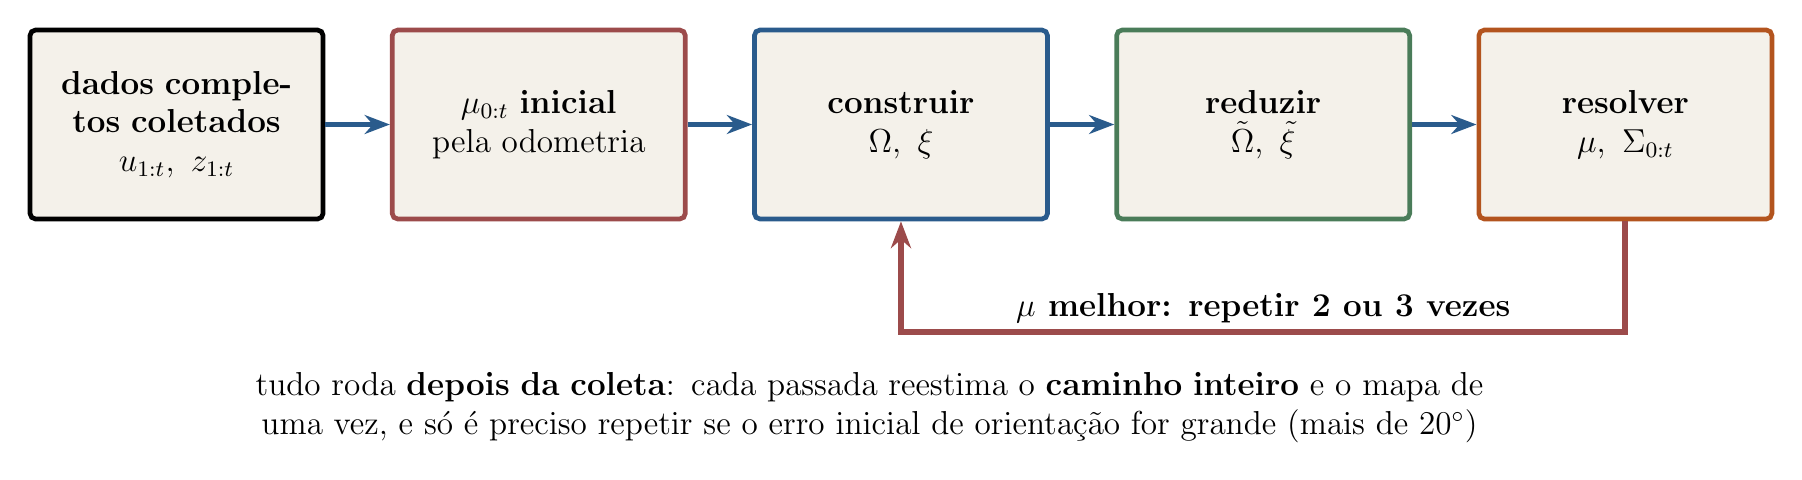
\begin{tikzpicture}[x=1cm,y=1cm]
\tikzset{k/.style={dbox, text width=3.3cm, minimum height=2.4cm, font=\large, line width=1.7pt}}
\node[k, draw=black] (z) at (1.8,4.0) {\textbf{dados completos coletados}\\ $u_{1:t},\ z_{1:t}$};
\node[k, draw=dred] (a) at (6.4,4.0) {$\mu_{0:t}$ \textbf{inicial}\\ pela odometria};
\node[k, draw=dblue] (b) at (11.0,4.0) {\textbf{construir}\\ $\Omega,\ \xi$};
\node[k, draw=dgreen] (c) at (15.6,4.0) {\textbf{reduzir}\\ $\tilde\Omega,\ \tilde\xi$};
\node[k, draw=dorange] (d) at (20.2,4.0) {\textbf{resolver}\\ $\mu,\ \Sigma_{0:t}$};
\draw[dtrans, line width=2pt, -{Stealth[length=3.2mm]}] (z) -- (a);
\draw[dtrans, line width=2pt, -{Stealth[length=3.2mm]}] (a) -- (b);
\draw[dtrans, line width=2pt, -{Stealth[length=3.2mm]}] (b) -- (c);
\draw[dtrans, line width=2pt, -{Stealth[length=3.2mm]}] (c) -- (d);
\draw[dred, line width=2.2pt, -{Stealth[length=3.4mm]}] (d.south) -- ++(0,-1.4) -| node[pos=0.25, above, font=\large\bfseries, text=black, fill=white, inner sep=2pt] {$\mu$ melhor: repetir 2 ou 3 vezes} (b.south);
\node[font=\large, text width=20cm, align=center] at (10.6,0.4) {tudo roda \textbf{depois da coleta}: cada passada reestima o \textbf{caminho inteiro} e o mapa de uma vez, e só é preciso repetir se o erro inicial de orientação for grande (mais de $20^\circ$)};
\end{tikzpicture}
\end{document}
